\section{Graf jadier}

V tejto časti popíšeme ako z jadier korekcie zostavíme kvázi de Bruijnov graf pre jedno čítanie. Vstupom je zoznam prekrytí medzi čítaniami a pre každé prekrytie aj zoznam jeho jadier. 

Začneme vytvorením zoznamu všetkých jadier z opravovaného čítania a z čítaní, ktoré sa s ním prekrývajú. Aby sme sa vyhli problémom súvisiacim so vzájomným prekrývaním jadier, rozbijeme dlhšie jadrá na postupnosť prekrývajúcich sa jadier pevnej dĺžky. Je vhodné použiť tú istú dĺžku ako bola minimálna dĺžka jadra v predchádzajúcej podkapitole. Pre každé jadro si algoritmus pamätá, či pochádza z opravovaného čítania, odhadovanú pozíciu a jej prislúchajúcu sekvenciu. Jadrá z opravovaného čítania budeme označovať silné. Tým, že jadrá sú pevnej dĺžky, ktorá neprekročí hodnotu 32, môžeme sekvencie reprezentovať ako celé čísla. V prípade, že prekrývajúce čítanie je z opačného vlákna, do zoznamu pridávame jadrá s obrátenou komplementárnou sekvenciou.

\paragraph{Odhadovanie pozície jadra}

Na rozdiel od nástroja LoRDEC, kde sa de Bruijnov graf zostavoval z iných čítaní, máme k dispozícii informáciu o pozícii jadier v rámci ich čítaní. Čím presnejšie odhadneme pozície jadier na opravovanom čítaní, tým prísnejšie podmienky môžeme nastaviť pri vytváraní hrán v grafe. Pre silné jadrá je pozícia jasne určená. V prípade jadier z prekrývajúcich sa čítaní môžu nastať dve situácie:

\begin{enumerate}[label={S.\arabic*}]
\item \label{jadro_medzi_dvomi_silnymi} Jadro sa nachádza medzi dvomi silnými jadrami
\item \label{jadro_medzi_silnym_a_okrajom_citania} Jadro sa nachádza na okraji čítania a silné čítanie má len na jednej strane.
\end{enumerate}

Pri odhadovaní pozície jadier prekrývajúceho sa čítania si do vyvažovaného stromu pre všetky silné jadrá uložíme dvojice (pozícia v prekrývajúcom sa čítaní, pozícia v opravovanom čítaní). Túto dátovú štrukturu potom použijeme na rozlíšenie medzi \ref{jadro_medzi_dvomi_silnymi} a \ref{jadro_medzi_silnym_a_okrajom_citania}. V prípade \ref{jadro_medzi_dvomi_silnymi} sa na vypočítanie pozície jadra použije priemer posunov najbližších silných jadier naľavo a napravo. V prípade \ref{jadro_medzi_silnym_a_okrajom_citania} použijeme len posun najbližšieho silného jadra. Názorná ukážka je na obrázku \ref{fig:odhadovanie_pozicie}. Červenou sú označené silné jadrá, zelenou je označený príklad situácie \ref{jadro_medzi_dvomi_silnymi} a modrou \ref{jadro_medzi_silnym_a_okrajom_citania}.

\begin{figure}
    \centering
    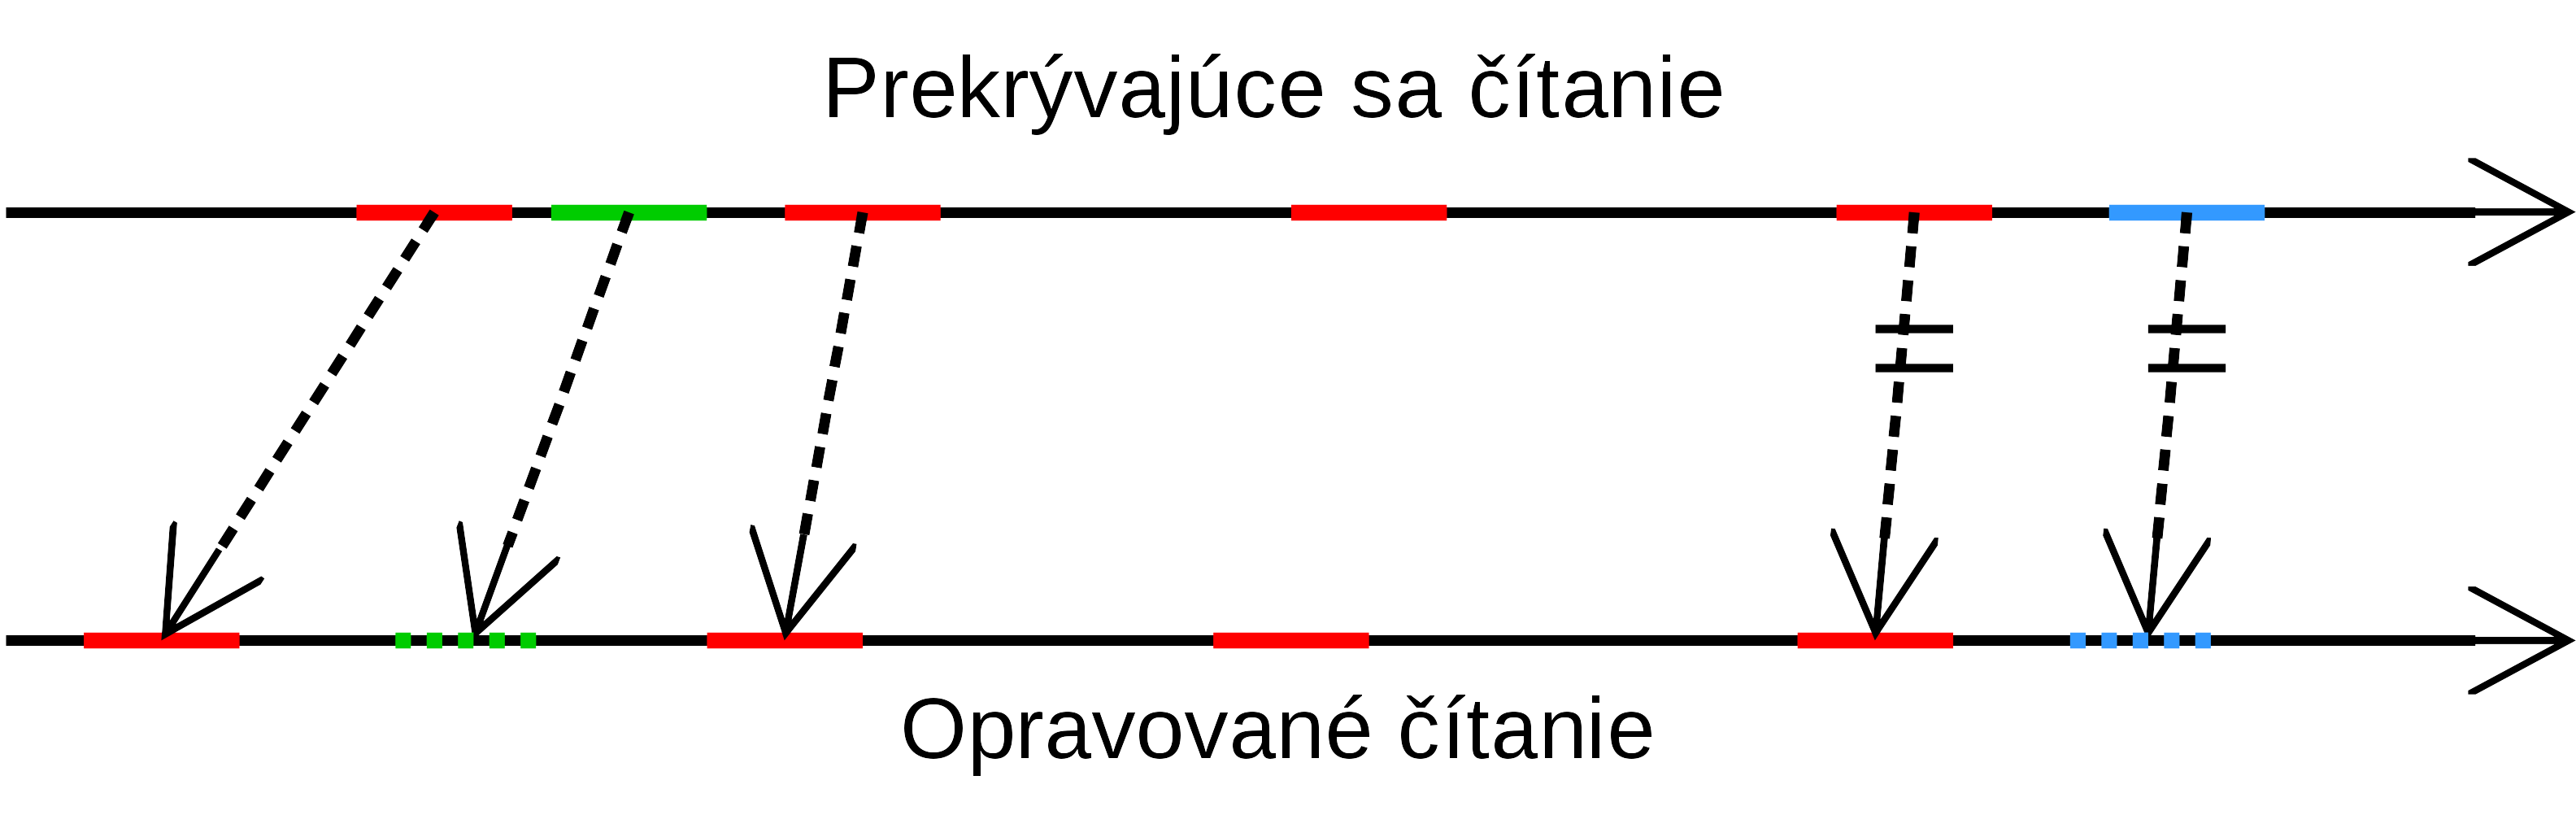
\includegraphics[width=0.8\textwidth]{images/odhadovanie_pozicie.png}
    \caption{Ukážka odhadovania pozícií jadier}
    \label{fig:odhadovanie_pozicie}
\end{figure} 

\paragraph{Odstraňovanie duplikátov}



\paragraph{Prekrytia jadier}